%% Template para dissertação/tese na classe UFBAthesis
%% versão 0.9.2
%% (c) 2005 Paulo G. S. Fonseca
%% (c) 2012 Antonio Terceiro
%% www.dcc.ufba.br/~terceiro/ufbathesis

\documentclass[msc, a4paper, classic, en]{ufbathesis}
\usepackage[utf8]{inputenc}
\usepackage[super]{nth}

%% Preâmbulo:
%% coloque aqui o seu preâmbulo LaTeX, i.e., declaração de pacotes,
%% (re)definições de macros, medidas, etc.

\title{A multi-view environment for markerless augmented reality}
\date{December \nth{15}, 2014}
\author{Caio Sacramento de Britto Almeida}
\adviser{Antônio Lopes Apolinário Júnior}
% \coadviser{<NOME DO(DA) CO-ORIENTADOR(A)>}

\begin{document}

% Folha de rosto
% FIXME: Check if 0007 is the right sequential number
\dmccfrontpage{MMCC-Msc-0007}
% Se seu trabalho não for uma tese de doutorado do DMCC, apague a linha
% acima e use \frontpage

%%
%% Parte pré-textual
%%
\frontmatter

% Portada (apresentação)
\dmccpresentationpage
% Se seu trabalho não for uma tese de doutorado do DMCC, apague a linha
% acima e use \presenationpage

% Ficha catalográfica
\authorcitationname{Sacramento de Britto Almeida, Caio} % e.g. Terceiro, Antonio Soares de Azevedo
\advisercitationname{Apolinário Jr., Antônio Lopes} % e.g. Chavez, Christina von Flach Garcia
\catalogtype{Thesis (master)} % e.g. ``Tese (doutorado)''
\catalogtopics{1. Multi-view environment. 2. Augmented reality. 3. Computer graphics} % e.g. ``1. Complexidade Estrutural. 2. Engenharia de Software''
% FIXME: Check the CDD
\catalogcdd{CDD 20.ed. 123.45} % e.g. ``CDD 20.ed. XXX.YY'' (esse número vai lhe ser dado pela biblioteca)
\catalogingsheet

% Termo de aprovação - exemplo
% Modifique com os membros da sua banca
\approvalsheet{Salvador, December \nth{15}, 2014}{
  \comittemember{Prof. Dr. Antônio Lopes Apolinário Júnior 1}{Federal University of Bahia - Brazil}
  \comittemember{Prof. Dr. Michelle Ângelo 2}{State University of Feira de Santana - Brazil}
  \comittemember{Prof. Dr. Rodrigo Silva 3}{Federal University of Juiz de Fora - Brazil}
}

% Agradecimentos
% Se preferir, crie um arquivo à parte e o inclua via \include{}
\acknowledgements
I would like to thank my family for all the support during all those years,
not only the time spent on the master program, but also during all my graduation.
Namely, first I would like to thank my brother, Rodrigo, for being my inspiration on following this career;
my twin sister, Thalita, for being my support of all times;
my parents, for the great education that was given to me;
my grandmother Lourdes; my girlfriend Jéssica; my friends; and specially my advisor Antônio Apolinário
for relying on me to make this work happen.

% Resumo em Português
% Se preferir, crie um arquivo à parte e o inclua via \include{}
%\resumo
% Palavras-chave do resumo em Português
%\begin{keywords}
%\end{keywords}

% Resumo em Inglês
% Se preferir, crie um arquivo à parte e o inclua via \include{}
\abstract
Augmented reality is a technology which allows 2D and 3D computer graphics to be aligned or registered with scenes of the real-world in real-time. This projection of virtual images requires a reference in the captured real image, which is often achieved by using one or more markers. But, there are situations where using markers can be unsuitable, like medical applications, for example. In this work, we present a multi-view environment, composed by augmented reality glasses and two Kinect devices, which doesn't use fiducial markers in order to run augmented reality applications. All devices are calibrated according to a common reference system, and then the virtual models are transformed accordingly too. In order to achieve that, two approaches were specified and implemented: one based on one Kinect plus optical flow and accelerometer data from augmented reality glasses, and another one based purely on two Kinect devices. The results regarding quality and performance achieved by these two approaches are presented and discussed, as well as a comparison between them.
\begin{keywords}
augmented reality, augmented reality glasses, kinect, transformation, optical flow, markerless
\end{keywords}

% Sumário
% Comente para ocultar
\tableofcontents

% Lista de figuras
% Comente para ocultar
\listoffigures

% Lista de tabelas
% Comente para ocultar
\listoftables

%%
%% Parte textual
%%
\mainmatter

% É aconselhável criar cada capítulo em um arquivo à parte, digamos
% "capitulo1.tex", "capitulo2.tex", ... "capituloN.tex" e depois
% incluí-los com:
% \include{capitulo1}
% \include{capitulo2}
% ...
% \include{capituloN}
%
% Importante: Use \xchapter ao invés de \chapter, conforme exemplo abaixo.

\xchapter{Introduction}{In this chapter I present the motivation, objectives and overview of this work.}
\section{Motivation}

Augmented reality has taken advantage from the progresses on the fields of multimedia and virtual reality, making feasible new forms of
interaction between humans and machines. Differently from virtual reality, that takes the user to a virtual environment, the augmented
reality keeps the user on his physical environment and takes the virtual environment to the user's space, allowing the interaction with
the virtual world, in a more natural manner and without needing training or adaptation \cite{1}. Many times, this interaction means
merging virtual images with images captured from a real environment.

One of the greatest challenges on the field of augmented reality is to determine, in real time, which virtual image to be displayed,
in which position and how it should be represented. In order to obtain an integration illusion between real objects and virtual objects,
the generated object should be aligned with the tridimensional position and orientation of the real objects \cite{2}. This can be achieved
by estimating the camera position.

On many situations, fiducial markers\footnote{A fiducial marker or fiducial is an object placed in the field of view of an imaging system which appears in the image produced, for use as a point of reference or a measure.} are used (often this is due to the real time requirements of the augmented reality applications) \cite{3} and are drawn in a way that they can be easily identified. Those markers need to be placed on the target scene and can achieve great results using just a few computational resources. Figure \ref{fig:fiducial_marker} shows the usage of a fiducial marker and a tridimensional object being projected over it.

\begin{figure}
\label{fig:fiducial_marker}
\centering
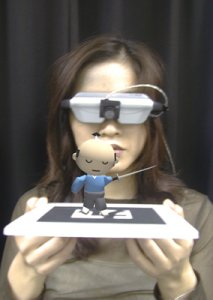
\includegraphics[width=0.3\textwidth]{images/fiducial_marker.png}
\caption{Fiducial marker used to represent a tridimensional model over it \cite{35}}
\end{figure}

However, besides requiring human interference on the scene, there situations where the usage of fiducial markers is not possible, feasible or comfortable for the target model. That is the case, for example, of medical applications on which this model is a patient. It's also possible to cite other limitations of fiducial markers, like, for example, occlusion (a virtual image could be not projected if the marker is not completely visible) and illumination (the intensity of light reflected by the marker could make it hard to be identified). Less common, there are approaches that replace fiducial markers \cite{6} \cite{7} by GPS, gyroscopes, accelerometers, cameras, among others \cite{3} \cite{8}. These approaches have the advantage of not requiring human interference on the scene (to put a marker or to move it around).

Depending on the way that a user sees the mixed world, augmented reality can be classified on two ways. When the user sees the mixed world pointing his eyes straight to the real positions with optical scene or video, this augmented reality is called \textit{immersive} or of \textit{direct vision}. On the other hand, when the user sees the mixed world by some device, like a monitor screen or projector, not aligned with the real positions, this augmented reality is \textit{non-immersive} or of \textit{indirect vision} \cite{1}.

This work proposes a multi-view environment for augmented reality, of direct vision, composed by two Kinects \cite{43} and augmented reality glasses, that allows a watcher visualize, in real time, virtual images merged with real images from the target model. In this approach, it's not intended to use any fiducial marker. Instead, it will be used a geometric approach based on the data captured by each Kinect. This proposed environment can be used, for example, on the medical field (real situations, education and training) or in other situation where a multi-view environment for markerless augmented reality is applicable. 

\section{Objectives}

The environment proposed on this work aims to contribute to augmented reality applications where virtual images need to be merged with real images in real time, without using fiducial markers, and considering the viewing angle of the observer and the position of the target object.

\subsection{Features}

Based on the study of related works, it was defined the following features that define the scope of the first version of the augmented
reality environment, graphically represented on Figure \cite{fig:diagram}:

\begin{figure}
\label{fig:diagram}
\centering
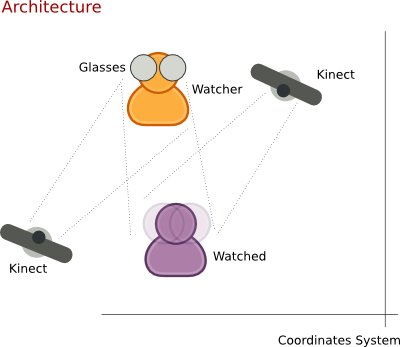
\includegraphics[width=0.3\textwidth]{images/diagram.png}
\caption{Global vision}
\end{figure}

\begin{itemize}
  \item There are two main elements on the environment, the observer and the target model;
  \item Observer and target model are positioned one in front of the other, with some restriction of minimum and maximum distance;
  \item The observer sees the combination of a real image with a pre-defined virtual image over the target model, through the augmented
        reality glasses;
  \item The observer and target model can move their heads, in a way that the virtual image adapts itself in real time to fit the new
        viewing angles;
  \item No fiducial marker is used.
\end{itemize}

The elements presented on this environment are the following:

\begin{itemize}
  \item Observer - He is the user of the system that wears a pair of augmented reality glasses and is positioned in front of the target model (which can be a human being, for example, or a static object). On a medical context, the observer would be a medical specialist, responsible for observing the patient and responsible for analyzing the combination of the real image (part of the patient body) with a virtual image (from magnetic resonance imaging or computed tomography). The observer is able to move his head.
  \item Augmented reality glasses - The augmented reality glasses are wore by the observer and have two cameras. The images captured from the target model will be merged with virtual images and displayed on the two lenses of these glasses. On one of the approches implemented by this work, the observer movimentation is determined from sensors present on the glasses: acceletometer, magnetometer and gyroscopes. Based on sensor data, it's possible to determine the variation on the orientation of the glasses, and so it's possible to know how much the observer has moved his head. This calculation returns values that define moviments on longitudinal axis, vertical axis and lateral axis. The virtual image should be reprojected in real time according to those movements.
  \item Target model - The target model (a human being, for example), is placed in front of the observer and doesn't use any kind of fiducial marker. The main goal is that the virtual image is placed over the target model. In order to calculate where and how the virtual image should be displayed, it's necessary to identify the position and orientation of the real object relative to the observer. This is done based on two sensors placed on the environment, where the first one captures data from the observer and the second one captures data from the target model.
  \item Sensors - Two sensors are placed on the environment and capture data from the observer and the target model (one for each). The information captured by the target model's sensor contains its model, that will be merged with the virtual image.
\end{itemize}

Each device presented on this multi-view (glasses and sensors) environment has its own coordinate system, but all information must be converted to a global coordinate system.

Since there are two sensors and one pair of augmented reality glasses, another objective is to implement two different approaches: one that
uses the augmented reality glasses to determine the observer's pose (based on data from accelerometer and magnetometer) and another one that uses a second Kinect device to determine the observer's pose based on a reconstruction of his model.

\section{Thesis overview}

The next chapter "Conceptual primer" describes some basic theory needed. It also describes the hardwares that are used by this work and how to calibrate them. After that, the "Related work" chapter presents some works related to this one, divided by subject. The third chapter, "Solution architecture", after the theory and related works were presented, explains the steps performed in order to implement the objectives of this work. The results of this implementation are presented on the chapter later, "Results", and finally the conclusions about those results are presented on the last chapter, "Conclusions", where possible future works are also listed.

\xchapter{Conceptual primer}{In this chapter I present the main concepts behind this work.}
\section{Augmented reality}

Augmented reality was born on the decade of 1990, to merge a virtual image or virtual environment with a real image or real environment. But only from the 2000s it became more popular, due to lower costs of hardware and software devices, and ready to be used on tangible and multimodal (voice, touch, gesture, etc.) applications \cite{4}. It can be considered the mixing of real and virtual worlds at some point of the continuum reality-virtuality, that connects completely virtual environments to completely real environments \cite{5}, like shown on Figure \ref{fig:cont}. It can also be considered a system that completes the real world with virtual objects, in a way that they seem to exist on the same space, respecting the following features:

\begin{figure}
\label{fig:cont}
\centering
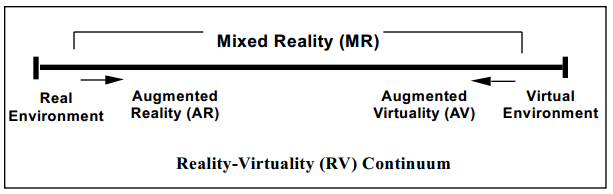
\includegraphics[width=0.5\textwidth]{images/cont.png}
\caption{The augmented reality is localized between the extremes of the reality-virtuality continuum}
\end{figure}

\begin{itemize}
  \item Real objects are mixed with virtual objects;
  \item Execution is interactive and on real time;
  \item Virtual and real objects are aligned;
  \item Applicable to all human sensory systems, including auditory, olfactory and somatosensory \cite{8}.
\end{itemize}

From a human-computer interaction perspective, the augmented reality can be considered a new way of interaction between humans and computers, and, on this aspect, it can be classified as direct vision or indirect vision.

\subsection{Direct or indirect vision}

Augmented reality is classified as \textit{direct vision} or \textit{immersive} when the user sees the mixed world pointing his eyes straight to the real position of the objects of interest, like shown on Figure \ref{fig:direct}.

\begin{figure}
\label{fig:direct}
\centering
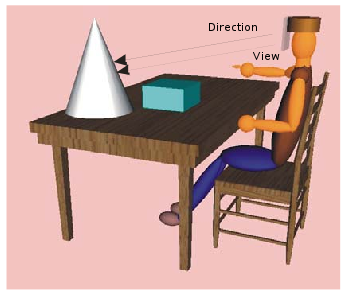
\includegraphics[width=0.5\textwidth]{images/direct.png}
\caption{Immersive augmented reality}
\end{figure}

On the direct vision, images from the real world can be seen with the naked eye ou brought by video, while the generated virtual images can be projected on the eyes, on the real scenario or mixed with the real world video. Immersive augmented reality can be implemented with optical helmets, for example \cite{1}.

\begin{figure}
\label{fig:indirect}
\centering
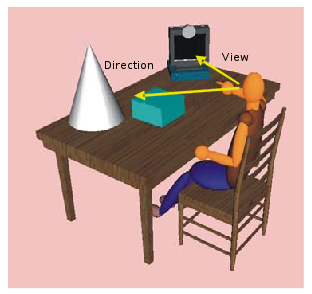
\includegraphics[width=0.5\textwidth]{images/indirect.png}
\caption{Non-immersive augmented reality}
\end{figure}

On the other hand, non-immersive augmented reality (indirect vision), happens when the user sees the mixed world through other output device, like a monitor screen, for example, not aligned with the real positions, as shown on Figure \ref{fig:indirect}. On this kind of vision, real and virtual images are merged and displayed as video to the user. It can be achieved by using cameras and projectors \cite{1}.

\subsection{Markers}

In order to identify the position where a virtual image should be rendered, two main approaches can be applied by augmented reality applications: one is to use fiducial markers, the other is not use them.

\subsubsection{Fiducial markers}

Fiducial markers are often implemented as square white cards with a black symbol printed (or drawn) on it, easy to be recognized, working like a barcode or QR code. Computer vision techniques are used to calculate the position of the real camera and its orientation relative to the markers, in a way that virtual objects can be projected over them.

Fiducial markers can assume other shapes besides a square card. The Figure \ref{fig:sticker} shows an example of a fiducial marker used on medical applications, similar to a sticker, which is fixed on the patient's skin. On these applications, augmented reality can be used for visualization and training on surgeries. It's possible to collect patient's data in real time, by using non-invasive sensors as the ones used for magnetic ressonance imaging and computed tomography. This dataset can be merged in real time with the real image of the patient \cite{12}.

\begin{figure}
\label{fig:sticker}
\centering
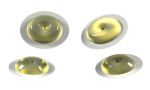
\includegraphics[width=0.5\textwidth]{images/sticker.png}
\caption{Example of fiducial marker used by medical applications}
\end{figure}

On motion capture systems, other kinds of markers can also be used, like, for example, the one described on \cite{24} and represented on Figure \ref{fig:helmet}. In order to estimate the pose, it uses a single camera and three spherical fiducial markers, which are also reflexive. Two of those markers are placed at the left and right sides of the actor, perpendicular to his ears. The third marker is placed on the same height as the other two, but in front of the actor. The markers have a color close to orange for high reflectance (in order to be easily recognized) and are supported by a structure made of carbon fiber (which is light).

\begin{figure}
\label{fig:helmet}
\centering
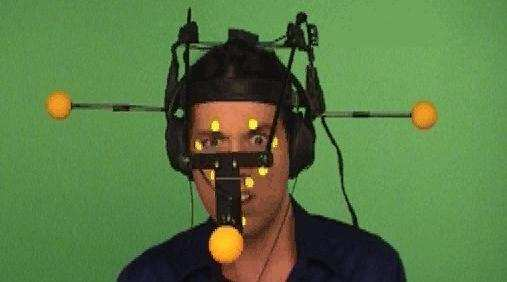
\includegraphics[width=0.5\textwidth]{images/helmet.png}
\caption{Example of fiducial marker for motion capture}
\end{figure}

Disadvantages of fiducial markers are listed on \cite{39}, for example, they are invasive (need to be placed on the scene or fixed on the target object), they have limited interaction (can't be moved around so much because it needs to still be visible and recognizable) and need to be printed or drawn before using and stored for future usage.

\subsubsection{Markerless}

Markerless augmented reality means that fiducial markers are not used on the scene. Instead, features from the target scene need to be used in order to estimate the camera pose and objects orientations.

Target detection based on computer vision has been extensively studied e successfully applied on augmented reality applications. On related computer vision literature, geometric primitives can be used for pose estimation, on most cases, points, segments, lines, edges of edge points, cones, cylinders, or a combination of two or more of those features.

Markerless augmented reality has the advantage of using parts of the real environment as targets and can even extract information from the environment to be used by the augmented reality system \cite{39}.

Avoiding markers leads to a much more effective augmented reality experience, but requires the implementation of several image processing or sensor function techniques, resulting in more complex algorithms and in higher computational resources \cite{shumaker2011virtual}.

\section{Cameras}

Many tasks on augmented reality deal with an imaging device. Usually this imaging device is a camera, which performs a mapping from a 3D world to a 2D image \cite{hanning2011high}. The problem called \textit{camera calibration} is the one that handles the determination of the parameters for this mapping.

\subsection{Calibration}

Camera calibration is a necessary step in 3D computer vision in order to extract metric information from 2D images. Much work has been done, by both the photogrammetry community and the computer vision community. Those techniques can be divided roughly into two categories: photogrammetric calibration (performed by observing a calibration object whose geometry in a 3-D space is known with very good precision) and self-calibration (does not use a calibration object, just move the camera in a scene and get its parameters) \cite{zhang2000flexible}.

Camera calibration means to determine the camera model parameters which fit best to the observed behavior of the actual camera \cite{hanning2011high}. So, it's necessary to measure the the distance of an observation to a given camera model. The determination of the optimal camera mapping concerning each of these distance functions defines a non-linear optimization problem, and as such, it depends on the initial value.

Ordinary cameras are very often modelled as pinhole cameras. A pinhole is an imaginary wall with a tiny hole in the center that blocks all rays except the ones that pass through this tiny center hole \cite{bradski2008learning}. Unfortunately, a real pinhole is not a good way to make images because it does not gather enough light for rapid exposure. This is why human eyes and cameras use lenses to gather more light than what would be available at a single point. This way, the simple geometry of the pinhole camera model is not enough and it also introduces distortion of the lens itself.

The camera coordinate system (CCS) is a Cartesian coordinate system defined by the principal plane: The x-axis and y-axis of the CCS determine the principal plane, the z-axis is given by the optical axis. The optical center of the lens determines the origin (0, 0, 0) of the CCS. Thus, in the camera coordinate system, the principal plane becomes ${ z = 0 }$ \cite{hanning2011high}.

Camera calibration is usually split up into two distinct parts, the intrinsic and extrinsic parameters, which will be covered on the following section.

\subsection{Parameters}

The process of camera calibration gives us both a model of the camera's geometry and a distortion model of the lens. Both compose the intrinsic parameters of the camera.

\subsubsection{Intrinsic parameters}

The intrinsic parameters are those that describe the internal workings  of the camera and consist of the focal length, the principal point, the skew coefficients and radial and tangential distortions \cite{tillapaugh2008indirect}. These values are needed to help to describe imperfections in the lens of the camera and give a mapping from camera reference frame to the image plane. The intrinsic parameters depend only on the camera itself, and so they just need to be found once, regardless the environment changes or not.

\subsubsection{Extrinsic parameters}

The extrinsic parameters, on the other hand, represent the viewpoint of the camera by a rigid transformation, which describes its position and orientation \cite{bajramovic2010self}. This part of the model is independent of the camera itself. The according parameters are called extrinsic, as they describe the relation between the camera and the world.

According to \cite{tillapaugh2008indirect}, the extrinsic parameters are those that are dependent on the environment. To relate an object's coordinate system to the world's coordinate system, a translation and a rotation matrix are needed. Therefore, the extrinsic parameters consist of these two matrices, so that a mapping from the world coordinate system to the camera reference frame can be found. Since the extrinsic parameters for the camera explain how the camera relates to the environment, if the camera changes position, the parameters have to be recalculated (differently from the intrinsic parameters as explained on the previous section).

The relation between world coordinate system and the camera reference frame can be described by the equation:

\begin{center}
$X_c = R_c \times X + T_c$
\end{center}

Where $X$ is a 3x1 vector that represents a point on the world coordinate space, $R_c$ is the extrinsic rotation matrix, $T_c$ is the extrinsic translation matrix and $X_c$ is a 3x1 vector in the camera reference frame. The rotation matrix is build from the combination of three single-axis rotation matrices:

\begin{center}

$R_{x}(\theta) =
\begin{bmatrix}
1 & 0 & 0 \\
0 & cos(\theta) & sin(\theta) \\
0 & -sin(\theta) & cos(\theta) \\
\end{bmatrix}$

\vspace{10mm}

$R_{y}(\phi) =
\begin{bmatrix}
cos(\phi) & 0 & -sin(\phi) \\
0 & 1 & 0 \\
sin(\phi) & 0 & cos(\phi) \\
\end{bmatrix}$

\vspace{10mm}

$R_{z}(\omega) =
\begin{bmatrix}
cos(\omega) & sin(\omega) & 0 \\
-sin(\omega) & cos(\omega) & 0 \\
0 & 0 & 1 \\
\end{bmatrix}$

\end{center}

The rotation matrix $R$ has the property that its inverse is its transpose, hence $R^TR = RR^T = I$, where $I$ is the identity matrix consisting of 1s along the diagonal and 0s everywhere else.

The translation vector $T$ is how it's possible to represent a shift from one coordinate system to another system whose origin is displaced to another location; in other words, the translation vector is just the offset from the origin of the first coordinate system to the origin of the second coordinate system \cite{bradski2008learning}. So, in order to shift from a coordinate system centered on an object to one centered at the camera, the appropriate translation vector is simply $T = origin_{object} - origin_{camera}$. Thus, a point in the object (or world) coordinate frame $P_o$ has coordinates $P_c$ in the camera coordinate frame: $P_c = R(P_o - T)$.

The extrinsic parameters can be represented by a final matrix called \textit{homegenous matrix}. It looks as follows:

\begin{center}
$\begin{bmatrix}
R & t \\
0 & 1 \\
\end{bmatrix}$
\end{center}

So, in order to convert from a world origin coordinate to a camera orientation coordinate system, only a single homogenous matrix needs to be used.

\subsection{Calibration approaches}

There are multiple ways to calibrate cameras. The most common way to perform the calibration is to have multiple points that have known relationship to each other in the world's coordinate system captured in an image from the camera \cite{tillapaugh2008indirect}. As explained previously, for the intrinsic parameters it does not matter how the points are related to the world coordinates, it's only important how they relate to each other. Such parameters consist of the horizontal and vertical focal lengths and the principal point of the camera and the skew. The skew is generally assumed to be zero \cite{furht2011handbook} for many cameras.

Various techniques were created to obtain accurate mappings, including vanishing points for orthogonal directions and calibration from rotation purely \cite{Medioni:2004:ETC:993884}, features extraction which can be lines or points, single-image or multiple-images configurations, different camera models, linear and non-linear algorithms, among many others \cite{Armangue00acomparative} \cite{clarke98}. Self-calibration is indeed feasible with simple image correspondences among frames, yet the participation of control points produces more robust calibration results, in closer agreement with object space constraints \cite{Douskos_automaticcalibration}.

The works by \cite{Tsai86} and \cite{zhang2000flexible} are extensively referenced and propose closed form solutions for the estimation of intrinsic and extrinsic parameters using 3D and 2D calibration patterns respectively. Camera calibration is a much discussed topic but the lack of robust algorithms for features detection difficults the construction of automatic calibration process \cite{gustavo}. Calibration pattern recognition is a hard task, where the lighting problems and high level of ambiguities are the principal challenges. For this reason, the algorithms often require user intervention for a reliable detection of the calibration points.

There are some tools available for automatic camera calibration. Two of the most popular ones are The Bouguet MatLab Toolbox \cite{matlab} and the OpenCV library \cite{opencv}. The former is an application that asks the user to define four extreme points that represent the area where an algorithm searches for the calibration points, given the number of rows and columns of the pattern. The latter is a very popular computer vision library that offers an automatic way to detect chessboard patterns in images by the \textit{findChessboardCorners()} function. The method performs successive morphological operators until a number of black and white contours are identified, subsequently the corners of the contours make up the calibration point set. The pattern is recognized only if all rectangles are identified. Figure \ref{fig:chessboard} shows how a person can use a chessboard in order to calibrate a camera using the OpenCV library.

\begin{figure}
\label{fig:chessboard}
\centering
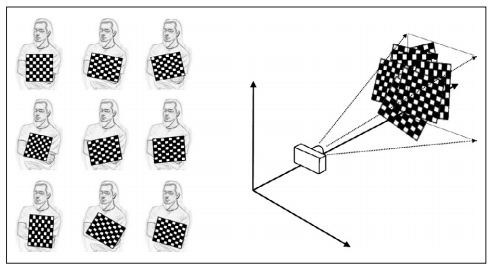
\includegraphics[width=0.5\textwidth]{images/chessboard.png}
\caption{Images of a chessboard being held at various orientations (left) provide enough information to completely solve for the locations of those images in global coordinates (relative to the
camera) and the camera intrinsics \cite{bradski2008learning}}
\end{figure}

As stated by \cite{arca}, the well-known algorithms for chessboard detection proposed by \cite{Tsai86} and \cite{zhang2000flexible} can achieve good calibration results since both of them are based on an initialization procedure that requires the precise corners positions of a calibration pattern (a chessboard, for example). Although the pattern to be detected is generally a simple object, the detection of its corners at subpixel precision is a very difficult task to be solved under uncontrolled acquisition conditions. At the state of art, most of the presented methods determine the positions of the chessboard corners by means of a two step processing scheme. At first the corners are detected with pixel precision, by means of edge detection methods; to increase the detection accuracy, the second step modifies their positions by the interpolation of the found borders. Those methods rarely reach a high accuracy, since the interpolation provides just a guess about the precise corners positions. Some authors try to improve the accuracy in the later steps of camera calibration, which increases computational cost, while others, like \cite{arca}, does not make any assumption on the orientation and scale of the chessboard and try to first find the chessboard, then determine the size of the squares and later on find the corners by using a simple statistical model.

\subsection{Multi-view}

Calibrating a multi-camera system accordingly means estimating the intrinsic and extrinsic parameters of all cameras \cite{bajramovic2010self}. Actually it is mainly concerned with estimating extrinsic parameters, since most approaches first compute intrinsic parameters individually for each camera. Extrinsic parameters are subsequently estimated given the intrinsic parameters.

The calibration task is usually formulated such that the world coordinate system may be chosen arbitrarily, which amounts to calibrate up to a rigid transformation of the whole system. Furthermore, if no metric measurements are used, the scale of the multi-camera system cannot be determined. This is the case if only correspondences between the cameras are used as input (of the extrinsic calibration) \cite{bajramovic2010self}.

According to \cite{hanning2011high}, the calibration of a stereo camera system is more than calibrating two camera separately: An additional constraint for the stereo camera system can be applied, since a calibration target is observed by both cameras.

So, in theory, calibration of a multi-camera system is possible by individually calibrating intrinsic and extrinsic parameters of all cameras involved with respect to the same world coordinate system using classical calibration methods. This just requires that all cameras observe a common calibration object or that a calibration object is moved to precisely known positions such that every camera can observe it. The first approach imposes very strict limitations on the allowable relative camera poses (relative orientation and position) or requires a very large calibration object, which is generally complicated \cite{Chen00widearea}.

Once cameras are calibrated, they are ready to register objects from a mixed reality scene. In general, traditional methods can be classified into three types: sensor-based methods, image-based methods and hybrid methods \cite{shumaker2011virtual}. The first two will be covered in the next sections; thr third, which is also applied by this work, won't be covered here since it's basically a combination of the first two methods.

\section{Sensor-based registration approach}

Three-dimensional (3D) reconstruction of an environment is an important problem that has received much attention in past decades. It can be defined as the process of capturing the shape and appearance of real objects \cite{chandra20123}. Recovering 3D surface structure of an object has been a central issue in computer vision. On the last years, with the launch of inexpensive RGBD sensors (notably the Kinect), applications based on sensor registration became cheaper and more feasible.

\subsection{Kinect}

\subsection{Registration}

\subsection{Transformation}

\section{Vision-based registration approach}

Registration based on sensors relies solely upon geometric information, for example, the spatial coordinates of the points in two clouds. As a result, environments that don't provide high geometric texture (for example, plane surfaces like a wall) can cause sensor tracking to fail. For such cases, a vision-based registration approach can be applied, by using the RGB information from the images \cite{kinectkanade}. 
\subsection{Optical flow}

Optical flow is a pattern that describes the apparent motion of objects, edges or surfaces on a visual scene caused by the relative motion between that object and an observer (a camera or the human eye) \cite{burton1978thinking}. This concept was first introduced by the psychology in order to describe the visual stimulus provided to animals moving on the world \cite{gibson1950perception}.

A fundamental problem in the processing of image sequences is the measure of the optical flow (or image velocity). The main objective is to compute an approximation to the 2D motion field - a projection of the 3D velocities of surface points onto the imaging surface - from spatiotemporal patterns of image density. Once computed, the measurements of image velocity can be used for many purposes, including object tracking \cite{opticalflow}.

The field of optical flow estimation is making big progresses as evidenced by the increasing accuracy of current methods on the Middlebury optical flow benchmark \cite{Scharstein:2002:TED:598429.598475}. After almost 30 years of research, these methods have obtained an impressive level of reliability and accuracy, by combining a data term that assumes constancy of some image property with a spatial term that models how the flow is expected to vary across the image \cite{opticalflow14}.

Differential methods belong to the most widely used techniques for optic flow computation in image sequences. They can be classified into local methods such as Lucas-Kanade technique or Bigun's structure tensor method, and into global methods such as the Horn/Schunck approach and its extensions. Often local methods are more robust under noise, while global techniques yield dense flow fields \cite{lkhs}.

Despite their differences, many of these techniques can be viewed conceptually in terms of three stages of processing \cite{opticalflow}:

\begin{itemize}
  \item Prefiltering or smoothing with low-pass/band-pass filter in order to extract signal structure of interest and to enhance the signal-to-noise ratio;
  \item The extraction of basic measurements, such as spatiotemporal derivatives (to measure normal components of velocity) or local correlation surfaces;
  \item The integration f these measurements to produce a 2D flow field, which often involves assumptions about the smoothness of the underlying flow field.
\end{itemize}

One of the most popular methods for computing the optical flow of an image is the Lucas-Kanade algorithm, which will be explained on the following section.

\subsection{Lucas-Kanade algorithm}

The Lucas-Kanade \cite{lk} algorithm is a differential method for computing the optical flow of an image \cite{kinectkanade}. The goal of Lucas-Kanade is to align a template image $T(x)$ to an input image $I(x)$ where $x = (x, y)^T$ is a column vector containing the pixel coordinates. If the Lucas-Kanade algorithm is being used to compute optical flow or to track an image from time $t = 1$ to time $t = 2$, the template $T(x)$ is an extracted sub-region (a window) of the image at $t = 1$ and $I(x)$ is the image at $t = 2$. Applications of the Lucas-Kanade algorithm range from optical flow and tracking to layered motion, mosaic construction and face coding. Numerous variations has been made to the original algorithm \cite{lk20}.

The basic idea of the Lucas-Kanade algorithm is based on three assumptions \cite{bradski2008learning}:

\begin{itemize}
  \item Brightness constancy: a pixel from the image of an object in the scene does not change in appearance as it (possibly) moves from frame to frame. For grayscale images (although Lucas-Kanade can also be done in color) this means that it's assumed that the brightness of a pixel does not change as it is tracked from frame to frame;
  \item Temporal persistence: the image motion of a surface patch changes slowly in time. In practice, this means the temporal increments are fast enough relative to the scale of motion in the image that the object does not move much from frame to frame;
  \item Spatial coherence: neighboring points in a scene belong to the same surface, have similar motion, and project to nearby points on the image plane.
\end{itemize}

Mathematically, the goal of the Lucas-Kanade is to minimize the sum of squared error between the two images, the template $T$ and the image $I$ warped back onto the coordinate frame of the template \cite{lk20}:

\begin{center}
  $\sum_{x}{[I(W(x;p))-T(x)]^2}$
\end{center}

Where $W(x;p)$ denote the parametrized set of allowed warps, where $p = (p_1,...,p_n)^T$ is a vector of parameters. The warp $W(w;p)$ takes the pixel $x$ in the coordinate frame of the template $T$ and maps it to the sub-pixel location $W(x;p)$ in the coordinate frame of the image $I$. In this context of optical flow computation, the warps $W(w;p)$ are the translations:

\begin{center}
$W(w;p) = \begin{matrix}
          x + p_1 \\
          y + p_2 \\
          \end{matrix}$
\end{center}

Where the vector of parameters $p = (p_1, p_2)^T$ is then the optical flow.

Warping $I$ back to compute $I(W(x;p))$ requires interpolating the image $I$ at the sub-pixel locations $W(x;p)$. The minimization is performed with respect to $p$ and the sum is performed over all of the pixels $x$ in the template image $T(x)$. Minimizing the expression is a non-linear optimization task even if $W(w;p)$ is linear in $p$ because the pixel values $I(x)$ are, in general, non-linear in $x$. In fact, the pixel values $I(x)$ are essentially un-related to the pixel coordinates $x$. To optimize the expression, the Lucas-Kanade algorithm assumes that a current estimate of $p$ is known and then iteratively solves for increments to the parameters $\Delta{p}$, so the expression is (approximately) minimized:

\begin{center}
  $\sum_{x}{[I(W(x;p + \Delta{p}))-T(x)]^2}$
\end{center}

With respect to $\Delta{p}$, and then the parameters are updated:

\begin{center}
  $p \gets p + \Delta{p}$
\end{center}

These steps are iterated until the estimates for the parameters $p$ converge.

The result of the algorithm is a set of optical flow vectors distributed over the image which give an estimation idea of the movement of objects in the scene, although some of those vectors will be erroneous \cite{raul}.

The Lucas-Kanade method can be applied in a sparse context because it relies only on local information that is derived from some small window surrounding each of the points of interest. The disadvantage of using small local windows in Lucas-Kanade is that large motions can move points outside of the local window and thus become impossible for the algorithm to find, which led to the development of the "pyramidal" Lucas-Kanade algorithm \cite{Bouguet00}, one of many approaches that have been used to improve the convergence rate and reduce the likelihood of falling into a local minimum.

One component in many algorithms is a coarse-to-fine strategy. The most common approach is to build image pyramids by repeated blurring and downsampling. So, optical flow is first computed on the top level (fewest pixels) and then upsampled and used to initialize the estimate at the next level \cite{dblk}, as shown on Figure \ref{fig:plk}. Computation at the higher levels in the pyramid involves far fewer unknowns and so is far faster. The initialization at each level from the previous level also means that far fewer interations are required at each level. Due to this, pyramid algorithms are usually faster than a single solution at the bottom level.

\begin{figure}
\label{fig:plk}
\centering
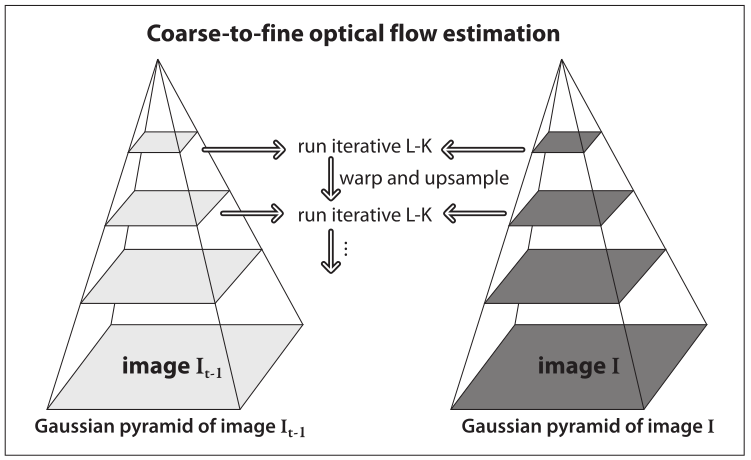
\includegraphics[width=0.5\textwidth]{images/plk.png}
\caption{Pyramid Lucas-Kanade optical flow: running optical flow at the top of the pyramid first
mitigates the problems caused by violating our assumptions of small and coherent motion; the motion estimate from the preceding level is taken as the starting point for estimating motion at the next layer down \cite{bradski2008learning}}
\end{figure}

The features to be tracked by the Lucas-Kanade algorithm can be manually defined or identified from an algorithm, like the popular one proposed by Shi and Tomasi \cite{shi}, called "good features to track", and implemented by the OpenCV library \cite{opencv}. The idea of this algorithm is a modification of the Harris Corner Detection \cite{harris}, which basically replaces Harris' scoring function. Figure \ref{fig:shi-harris} shows the feature points on the same input image as identified by both algorithms.

\begin{figure}
\label{fig:shi-harris}
\centering
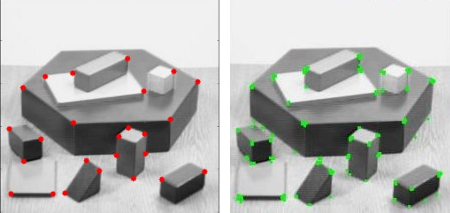
\includegraphics[width=0.5\textwidth]{images/shi-harris.png}
\caption{The same input image being used for features identification by Shi-Tomasi algorithm (red dots) and by Harris Corner Detector (green dots)}
\end{figure}

So, the Lucas-Kanade algorithm, applied over a good set of feature points, is an efficient method for obtaining optical flow information at interesting points in an image and works for moderate object speeds.

\xchapter{Related works}{In this chapter I present some related works.}
Cover all the related works, with multiple Kinects, optical flow, markerless augmented reality, medical applications, multi-view environment, reconstruction, etc.
\section{Markerless augmented reality}
\section{Multiple Kinects}
\section{Multi-view environment}

\xchapter{Solution architecture}{In this chapter I explain in details the steps performed in order to implement the objective of this work.}
\section{Environment}
Technologies, machines, SOs, etc.
\section{Calibration}
\subsection{Augmented reality glasses calibration}
\subsection{Initial calibration between Kinects}
\subsection{Initial calibration between Kinect and glasses}
\section{Communication}
Network, sockets, etc.
\section{Transformations}
\section{Method 1: Glasses accelerometer and one Kinect}
Cover Lucas-Kanade algorithm, etc.
\section{Method 2: Two Kinects}
Talk about performance of two Kinfus fighting for a single GPU.
\section{Hybrid approach}
When optical flow has just a few feature points, we switch to the second Kinect.

\xchapter{Result}{In this chaper I present the results of the procedure explained in the previous chapter.}
\section{Scope}
Talk about error propagation.
\section{Analysis}
Talk about performance and alignment results.
\section{Comparison}
Compare methods 1 and 2 with regards to performance and quality.

\xchapter{Conclusions}{In this chapter I discuss the conclusions of this work and list some possibilities of future works.}
\section{Future work}

\backmatter

% Apêndices
% Comente se não houver apêndices
\appendix

% É aconselhável criar cada apêndice em um arquivo à parte, digamos
% "apendice1.tex", "apendice.tex", ... "apendiceM.tex" e depois
% incluí-los com:
% \include{apendice1}
% \include{apendice2}
% ...
% \include{apendiceM}


% Bibliografia
% É aconselhável utilizar o BibTeX a partir de um arquivo, digamos "biblio.bib".
% Para ajuda na criação do arquivo .bib e utilização do BibTeX, recorra ao
% BibTeXpress em www.cin.ufpe.br/~paguso/bibtexpress
\bibliographystyle{abnt-alf}
\bibliography{template}

%% Fim do documento
\end{document}
